\paragraph{Pipeline verification without model calls.} To check that splitting, merging and scoring do not themselves change the outcome, DevBench's reference implementation is cut into the fragments that each agent of each condition would own, merged by the same deterministic merge step as agent output, and scored. Every condition must reach the score of the unsplit reference code, and every condition does (geotext 9/9; hone 12/12; lice 31/31; particle-swarm-optimization 6/6; stocktrends 9/9, for G2, G4, GC, G6 and G7). A smoke run before the pilot exposed four defects in the harness, all fixed before any comparison and applied identically to every condition: a missing package installer on the host, subclasses merged before their base class, traceability markers written by the model without a comment sign, and classes split across agents losing methods in the merge. These changes are listed as deviations in the released pre-registration folder.

\paragraph{Model selection.} The model was chosen before the pilot by a probe that runs only the single-agent condition (G2), so the choice cannot favor any way of splitting. The decision rule was written down before the probe: switch to a larger reasoning model only if it passes at least three more tests in total, and add DevBench's sequence diagram to every agent's input only if it does not lower the score. Neither condition was met (Table~\ref{tab:probe}): the larger model passed the same number of tests at about five times the tokens, and the sequence diagram did not help, so the pilot keeps the cheaper model and the original inputs.



\paragraph{Pilot (Python projects).} Table~\ref{tab:pilot} reports three runs per condition. Correctness did not differ between conditions on any project: on geotext every condition passed the same 0 of 9 tests in every run; on lice every condition passed the same 0 of 31 tests in every run; on particle-swarm-optimization every condition passed the same 4 of 6 tests in every run; on stocktrends every condition passed the same 1 of 9 tests in every run. Scores sit at or near zero on three projects (a floor effect), so the pilot cannot separate the conditions on correctness. Costs did differ (Figure~\ref{fig:pilot}). On every project for which the criterion recommends a single agent (geotext, lice, particle-swarm-optimization), the single agent used fewer tokens than random and one-agent-per-class teams (34--90\% fewer; exact one-sided permutation tests over runs, p = 0.05 for each comparison, the smallest value attainable with three runs per condition) and exchanged no messages; per-project values are in Table~\ref{tab:pilot}. On stocktrends ($k^\ast$ = 3) the criterion team used 14,162 tokens per run against 13,511 for random teams of equal sizes (+5\%, within the pre-registered 10\% margin) and 17,879 for one agent per class and Infomap, which formed the same team (21\% fewer), and exchanged 2 messages against 1 for random teams and 3 for one agent per class. Figure~\ref{fig:teams} shows run 0 of the criterion team and of a random team on stocktrends: the criterion team keeps every class with one agent, so cohesion inside agents is high (0.44--0.75) and coupling between them low (0.00--0.10), whereas the random team spreads classes over agents (cohesion 0.12--0.28, coupling 0.20--0.38); both nevertheless passed the same test, which illustrates that structural quality alone did not translate into correctness on this task. Under the pre-registered rules the pilot is a provisional NO-GO: the criterion team did not pass more tests than random teams on the only scored multi-agent project (a tie, with no strict win); the other rules hold: the criterion team stays within the 10\% token margin of random teams and the single agent is at least as correct as split teams where $k^\ast$ = 1; the decision becomes final once the C++ and Java pilot projects are scored. Experiment 1b, registered before its runs, adds fresh projects for which the criterion recommends one agent: the single agent used fewer tokens than both split teams on every one of the 3 such projects (H3a), and it was at least as correct as the split teams on 1 of the 1 projects on which any condition passed a test (H3b). Inspection of the failing tests shows two causes that affect every condition alike: tests that require identifiers appearing in neither the requirements nor the design (for example, a class constant or a default argument named only in a test), and errors in the model's own code, such as wrong numeric logic or a module that fails at import. The harness itself is not a cause, since the reference code passes every test after the same split and merge. The main study therefore needs tasks on which the model passes a meaningful share of tests; Section~\ref{sec:discussion} discusses this. The whole Python pilot used 408,518 tokens, which cost less than one US dollar with this model.



\begin{figure}[t]\centering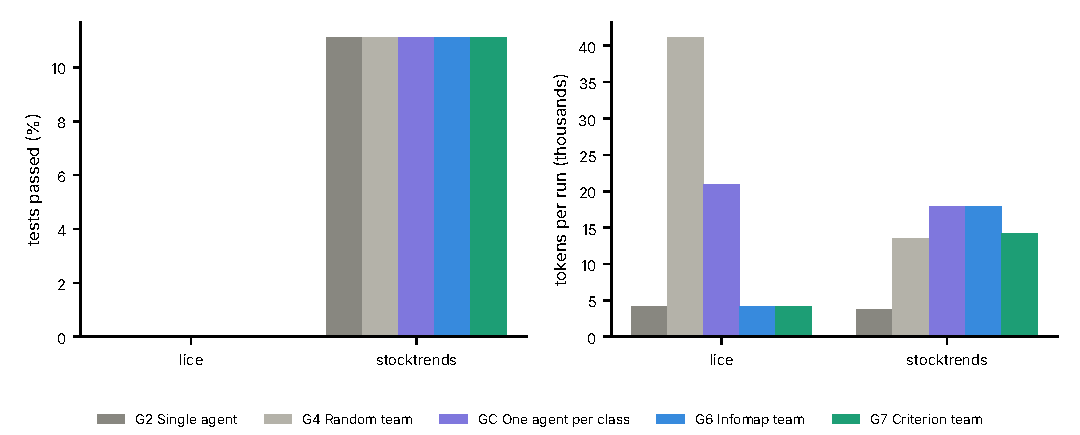
\includegraphics[width=\linewidth]{figures/pilot.pdf}
\caption{Pilot: tests passed (left) and tokens per run (right) for each condition.}\label{fig:pilot}\end{figure}



\textbf{\emph{Main study (planned, pre-registered):}} The confirmatory tests follow the pilot. H1 uses a paired Wilcoxon signed-rank test over tasks with Holm correction and reports bootstrap confidence intervals; H2 correlates cut weight with logged messages per agent pair (Spearman); H3 cross-tabulates the split or no-split decision against the empirically better choice; and H4 repeats H1 with designs extracted from the requirements. The study adds the C++ and Java DevBench projects, further multi-agent tasks to reach the roughly 36 that the power analysis requires, and a second model from a different model family.
